\documentclass[11pt]{article}

\usepackage[margin=1in]{geometry}
\usepackage{amsmath,amssymb}
\usepackage{booktabs}
\usepackage{array}
\usepackage{graphicx}
\usepackage{hyperref}

\title{Scalar Continuum Control, Harmonic-Coexact Sector Separation, and a Bounded Roadmap Toward Continuum Physics on HAOS-IIP}
\author{Tomislav Rupi\'c \\ Independent Researcher}
\date{April 2026}

\begin{document}
\maketitle

\begin{abstract}
This paper freezes the current April 2026 continuum-facing state of the HAOS-IIP repository as one bounded synthesis release. The question is narrow. It is not whether spacetime, gauge theory, or field ontology has emerged. It is whether the already frozen operator family now supports a stronger scalar continuum contract and whether the vector-sector evidence survives a stricter full-spectrum test. The answer is asymmetric. On the scalar side, the local kernel-induced node operator now remains convergent not only on the clean cubic interior scan, but also on weakly perturbed three-dimensional point sets and explicit homogeneous Dirichlet and Neumann boundary controls. On the vector side, the projected low transverse branch continues to track continuum ordering after $n^2$ rescaling, but the full low $L_1$ floor remains harmonic, and the direct harmonic-to-coexact gap stays finite through the tested $n=28$ window. Defects compress this separation and can pull the coexact candidate deeper into the low window, but they do not collapse it into the actual low propagating floor. The bounded conclusion is therefore explicit: the scalar continuum contract now passes in the tested local regime, while the vector continuum contract remains open. The paper closes by defining a numbered future program from harmonic-floor resolution through effective-law closure, geometry closure, and universality.
\end{abstract}

\section{Scope}

This paper is a synthesis release, not a new phase contract. It compresses the current CP1 through CP2c continuum-scaling work on top of the already frozen operator hierarchy and earlier continuum-facing papers. In particular, it inherits without change:
\begin{itemize}
\item the kernel-induced node operator $L_0 = D-W$;
\item the edge operator $L_1 = d_0 d_0^* + d_1^* d_1$;
\item the restricted transverse operator
\[
T = d_1^* d_1 \big|_{\ker(d_0^*) \cap (\mathcal{H}^1)^\perp};
\]
\item the earlier restricted-sector continuum reconstruction reported in Paper 02.1;
\item the frozen branch-local hierarchy and proto-continuum sketch reported in Paper 44.1.
\end{itemize}

The present release adds no new dynamics, no quantization rule, no metric ontology, and no physical correspondence claim. It asks only what is now established after the stricter April 12, 2026 scalar and vector scans.

\section{Current Question}

The repository already contained two continuum-facing ingredients before the present synthesis:
\begin{enumerate}
\item a restricted transverse branch whose low spectrum was consistent with a continuum transverse ordering and an almost gapless effective fit;
\item a late-phase proto-continuum sketch showing refinement-ordered behavior of selected frozen observables.
\end{enumerate}

Those were meaningful, but they did not close the stronger question ``scale HAOS-IIP to continuum physics.'' In the current repository, the narrow operational meaning of that phrase is:
\begin{quote}
the same frozen operator family should admit a refinement-stable, sector-resolved, perturbation-robust effective continuum description whose leading observables survive controlled changes of resolution, background, and boundary handling.
\end{quote}

This paper addresses only the first two gates of that ladder:
\begin{enumerate}
\item CP1: scalar continuum control on more than one substrate family;
\item CP2: vector-sector separation strong enough to distinguish a true coexact low branch from harmonic or topological low modes.
\end{enumerate}

\section{CP1: Scalar Continuum Contract}

\subsection{Setup}

The scalar scan extends the earlier cubic interior test in three ways:
\begin{enumerate}
\item cubic interior baseline on $n=9,11,13,17,21$ with kernel widths $\varepsilon_k = c_\varepsilon h^2$ and $c_\varepsilon \in \{0.5,1.0,2.0\}$;
\item weakly jittered point sets on $n=11,13,15,17$ with interior jitter amplitude $0.04h$, fixed seed $42$, and the same local kernel weights recovered by local quadratic fitting;
\item full-domain reflected boundary controls with odd reflection for homogeneous Dirichlet data and even reflection for homogeneous Neumann data.
\end{enumerate}

The operator is normalized by the discrete second moment,
\[
\widehat{L}_h = -\frac{2}{\mu_2 h^2} L,
\]
and compared against the continuum Laplacian on quadratic, trigonometric, and Gaussian test functions. The scalar question remains purely operator-level: does the same local kernel support stable Laplacian-type control under refinement, mild geometric disorder, and explicit boundary handling?

\subsection{Results}

The cubic baseline remains intact, and the new point-set and boundary controls pass in the bounded local-kernel regime. The main convergence orders are summarized in Table~\ref{tab:cp1-orders}.

\begin{table}[t]
\centering
\small
\begin{tabular}{lccc}
\toprule
Diagnostic & $c_\varepsilon=0.5$ & $c_\varepsilon=1.0$ & $c_\varepsilon=2.0$ \\
\midrule
Cubic trigonometric order & 1.9825 & 1.8579 & 1.3770 \\
Cubic Gaussian order & 1.8035 & 1.2495 & 0.3316 \\
Dirichlet boundary order & 1.9825 & 1.9680 & 1.9405 \\
Neumann boundary order & 2.1902 & 2.1756 & 2.1482 \\
\bottomrule
\end{tabular}
\caption{CP1 scalar convergence orders in the stamped April 12, 2026 scalar run. The broad-kernel regime remains the weak point, while the local regime stays clean across all tested controls.}
\label{tab:cp1-orders}
\end{table}

The point-set control gives a narrower but still positive result:
\begin{itemize}
\item quadratic reproduction stays at machine precision, with maximum $L^2$ error $5.96\times 10^{-14}$ across the scan;
\item trigonometric convergence on the jittered point sets is $p=1.8223$ at $c_\varepsilon=0.5$;
\item Gaussian convergence on the same point sets is weaker but still positive at $p=1.0611$;
\item valid stencil fraction remains above $0.975$ with average neighbor count near $20$--$21$.
\end{itemize}

The scalar verdict is therefore stronger than the earlier cubic-only March note. In the tested local regime, the same node operator now admits bounded continuum control on:
\begin{enumerate}
\item the clean cubic interior scan;
\item a weakly perturbed three-dimensional point-set control;
\item explicit homogeneous Dirichlet and Neumann boundary families.
\end{enumerate}

This is still not a metric claim, a curvature claim, or a universality claim across arbitrary kernels. It is a contract-level scalar operator result in a bounded regime.

\begin{figure}[t]
\centering
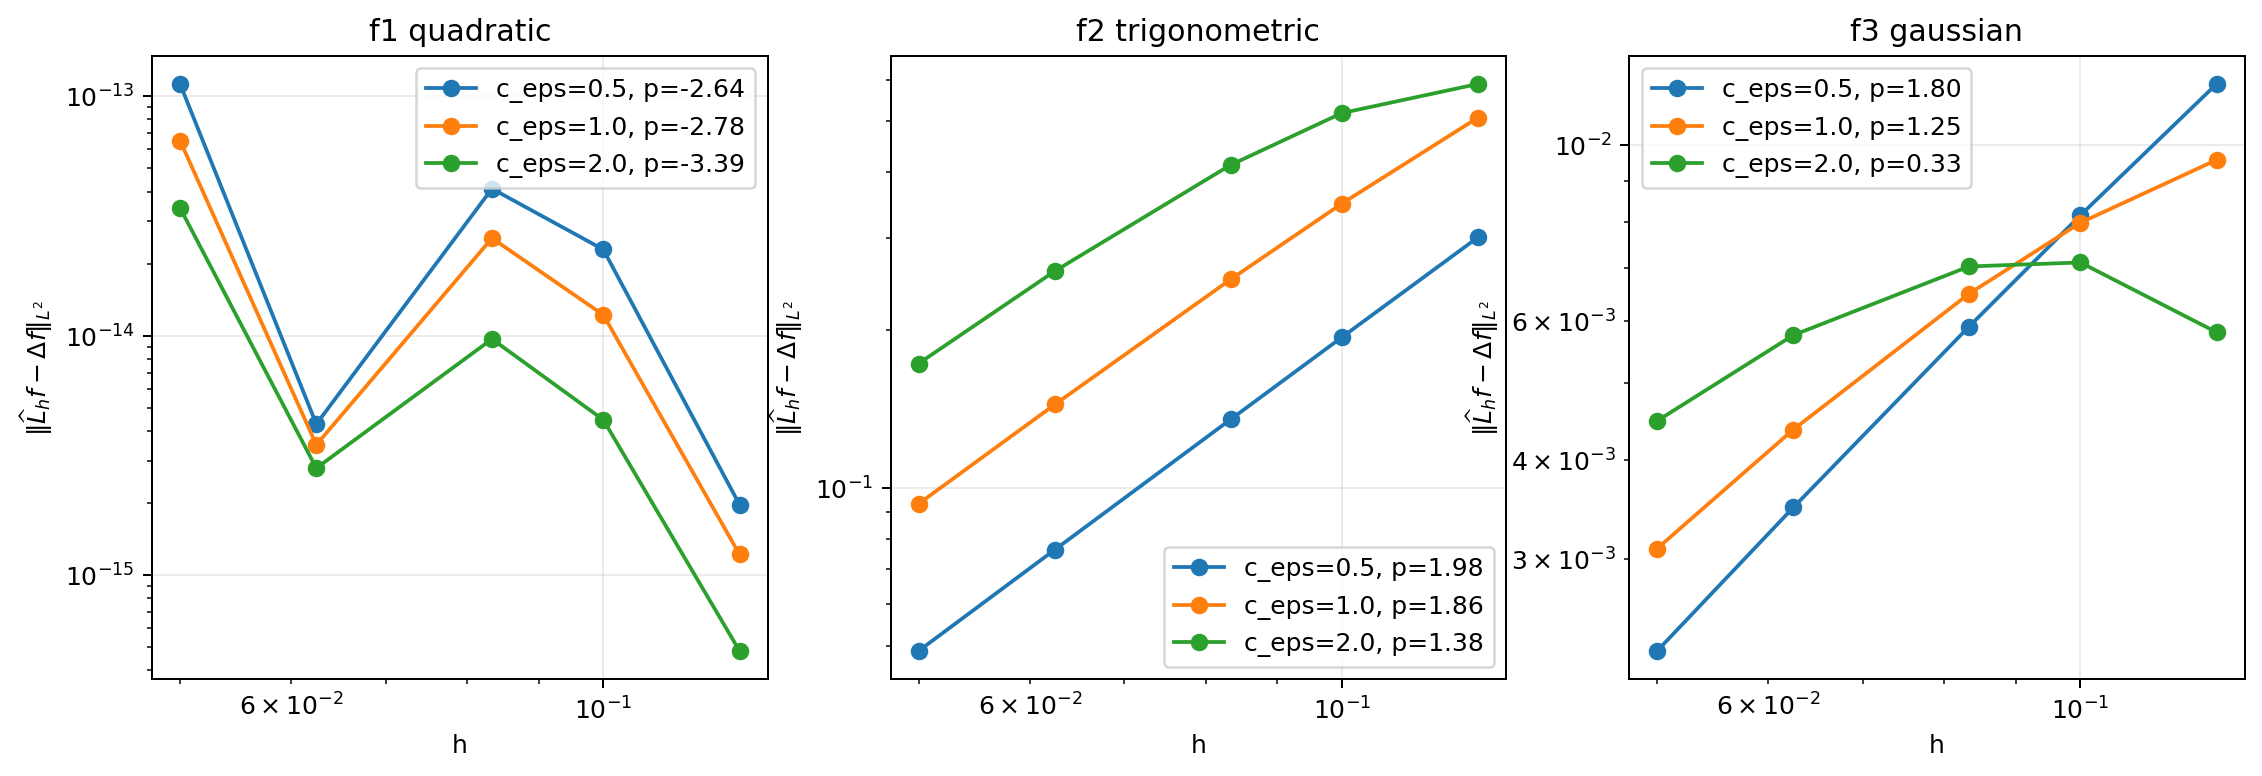
\includegraphics[width=0.32\linewidth]{../plots/20260412_101326_operator_error_vs_h.png}
\hfill
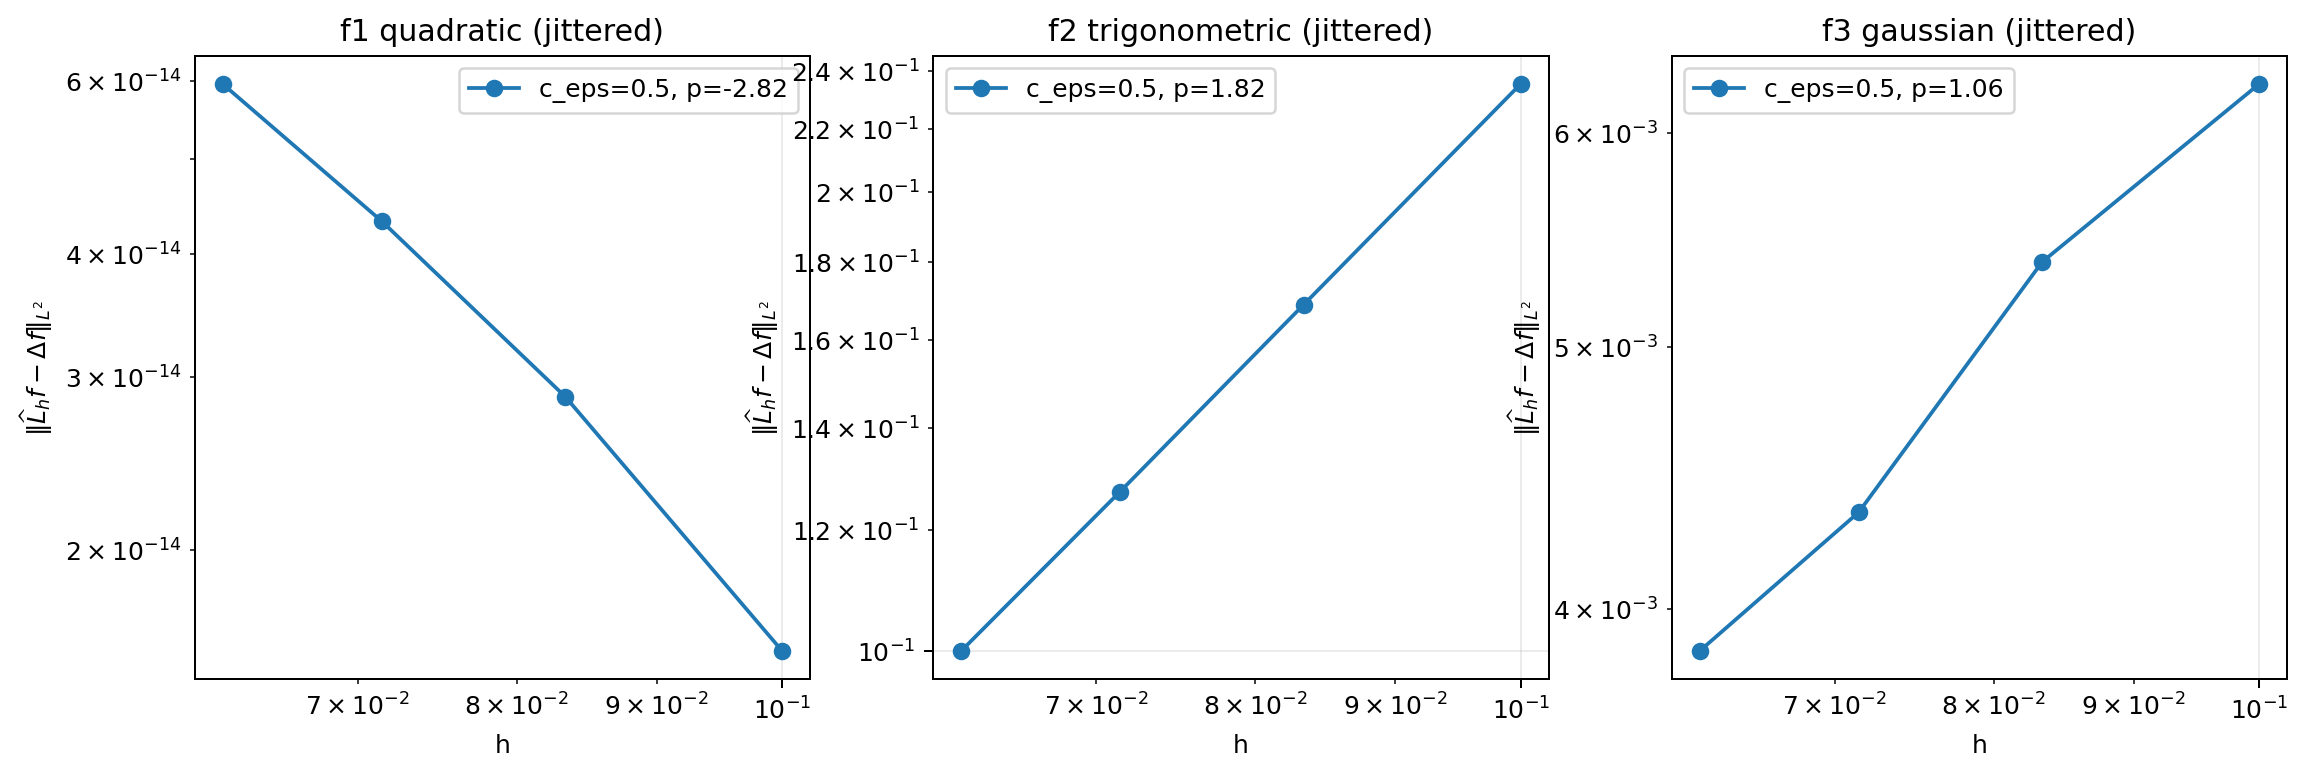
\includegraphics[width=0.32\linewidth]{../plots/20260412_101326_point_set_operator_error_vs_h.png}
\hfill
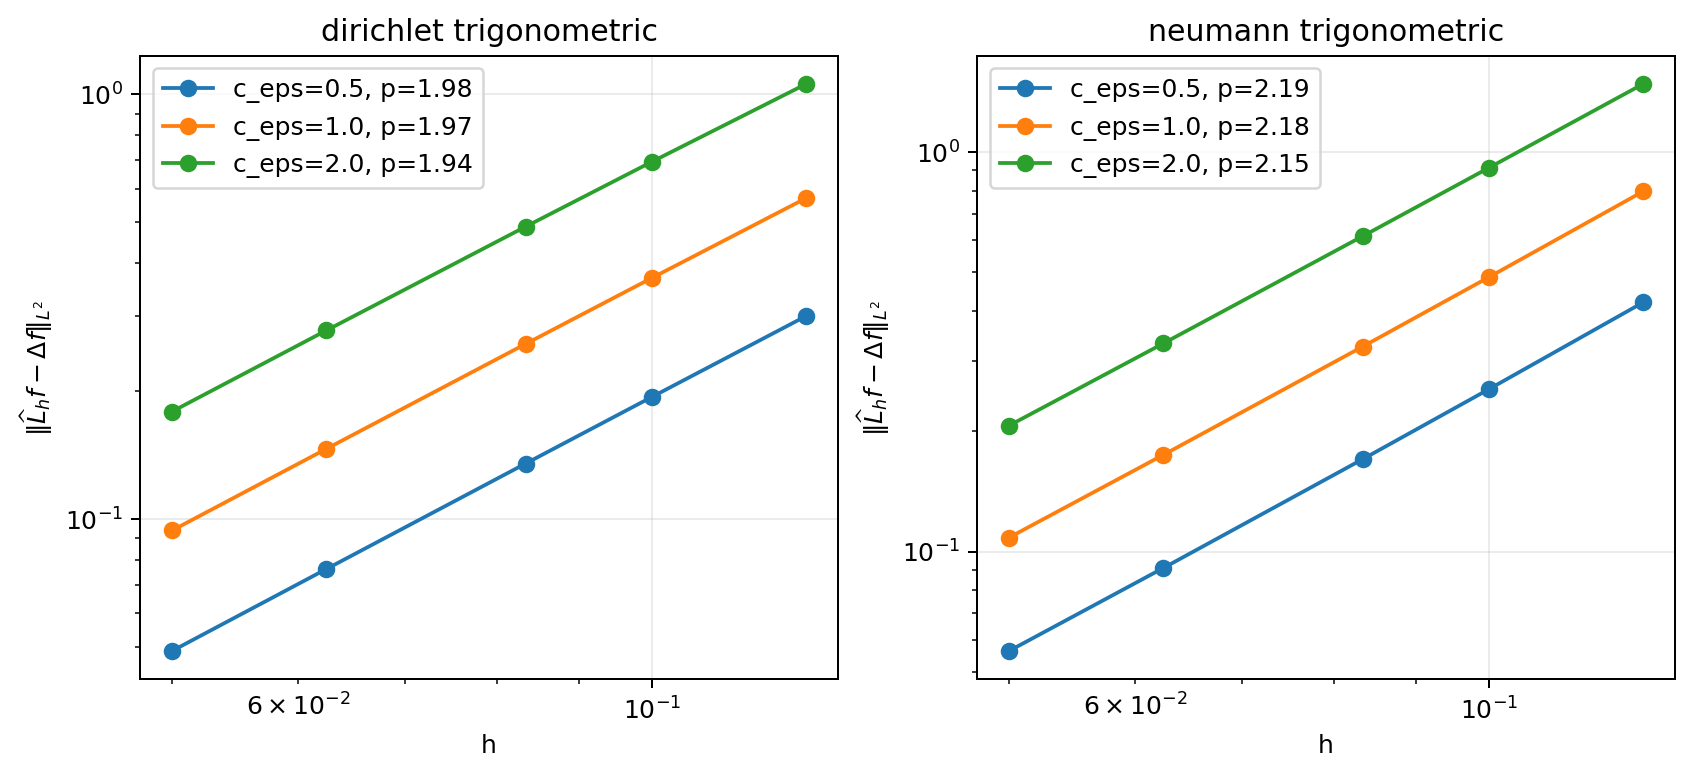
\includegraphics[width=0.32\linewidth]{../plots/20260412_101326_boundary_condition_error_vs_h.png}
\caption{CP1 scalar diagnostics. Left: cubic interior convergence. Center: weakly perturbed point-set convergence in the local regime. Right: reflected boundary-condition convergence for homogeneous Dirichlet and Neumann controls.}
\label{fig:cp1}
\end{figure}

\section{Why CP2 Had To Be Stricter Than Paper 02.1}

Paper 02.1 established a real restricted transverse result on the frozen architecture. In the clean periodic branch, the low restricted fit
\[
\lambda_k \approx c_{\mathrm{eff}} |q_k|^2 + m_{\mathrm{eff}}
\]
gave stable stiffness values
\[
c_{\mathrm{eff}} = 37.9206,\ 38.5949,\ 38.9108,\ 39.0834
\]
with numerically vanishing fitted gap in the tested restricted sector. That result remains meaningful. The April 2026 vector work does not revoke it.

But a stronger question remained open:
\begin{quote}
does the full low $L_1$ spectrum itself already sit in that same coexact continuum-like sector, or is the projected transverse branch hiding above a harmonic or topological floor?
\end{quote}

That stricter question is what CP2 through CP2c were designed to answer. The new diagnostics therefore record not only the projected spectrum, but also:
\begin{itemize}
\item the harmonic and coexact fractions of the true low full-spectrum modes;
\item the first strong coexact candidate in the scanned full window, using the threshold coexact fraction $\geq 0.8$;
\item the harmonic-to-coexact gap
\[
g_{\mathrm{hc}} = n^2(\lambda_{\mathrm{candidate}}-\lambda_{\mathrm{floor}});
\]
\item candidate localization near defects and the ratio between the projected floor and the selected full-spectrum coexact candidate.
\end{itemize}

\section{CP2: Initial Full-Spectrum Sector Split}

\subsection{Restricted band versus full low floor}

The first full CP2 comparison kept the restricted continuum diagnostic but added explicit full-spectrum sector tests on $n=12,16,20$ for the baseline, puncture, line-defect, and flux-tube backgrounds. The restricted branch still follows continuum ordering after $n^2$ rescaling, with first-ten relative spectrum errors:
\begin{itemize}
\item baseline: $0.2189$ at $n=12,16,20$;
\item puncture: $0.0526$, $0.0251$, $0.0131$;
\item line defect: $0.0180$, $0.0103$, $0.0066$;
\item flux tube: $0.1592$, $0.1627$, $0.1647$.
\end{itemize}

The key new point is that this projected success does \emph{not} coincide with the true low full-spectrum floor. In every tested branch, the lowest full mode remains harmonic-dominated. The largest-size CP2 comparison is summarized in Table~\ref{tab:cp2-n20}.

\begin{table}[t]
\centering
\small
\begin{tabular}{lccccc}
\toprule
Branch & rel. err. (10) & low harmonic frac & candidate $j$ & threshold hit & restricted/candidate \\
\midrule
baseline & 0.2189 & 1.000 & 8 & no & 1.000 \\
puncture & 0.0131 & 1.000 & 3 & yes & 1.000 \\
line defect & 0.0066 & 1.000 & 3 & yes & 1.000 \\
flux tube & 0.1647 & 1.000 & 8 & yes & 0.949 \\
\bottomrule
\end{tabular}
\caption{Largest-size CP2 comparison at $n=20$. The restricted branch continues to look continuum-like, but the true lowest full $L_1$ mode remains harmonic in every branch.}
\label{tab:cp2-n20}
\end{table}

The correct bounded reading is therefore asymmetric:
\begin{enumerate}
\item the projected coexact branch is real and still organizes like a continuum transverse spectrum;
\item the actual low $L_1$ floor is not yet that branch.
\end{enumerate}

\begin{figure}[t]
\centering
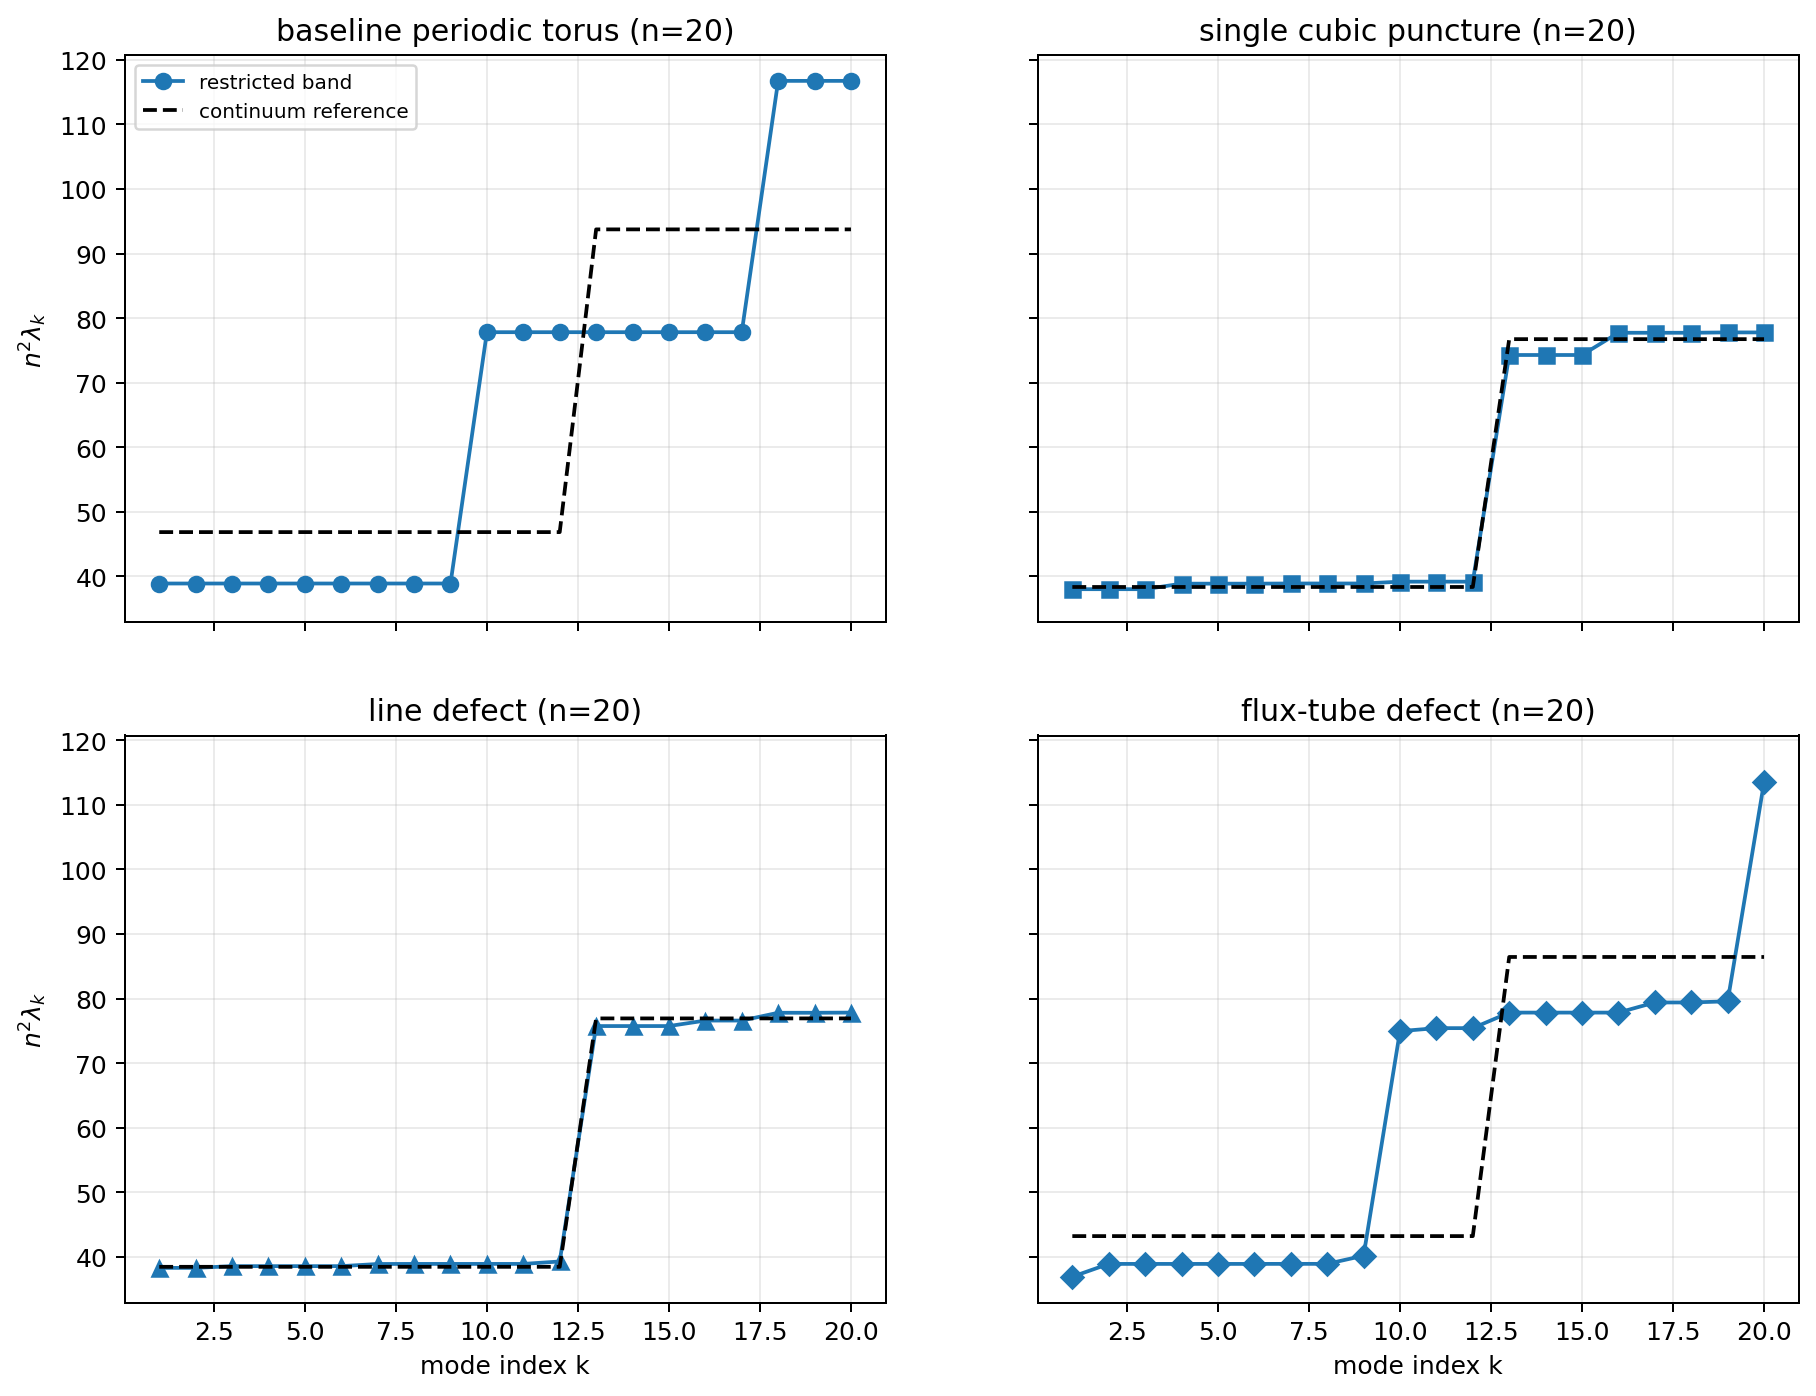
\includegraphics[width=0.48\linewidth]{../plots/20260412_141530_transverse_continuum_comparison.png}
\hfill
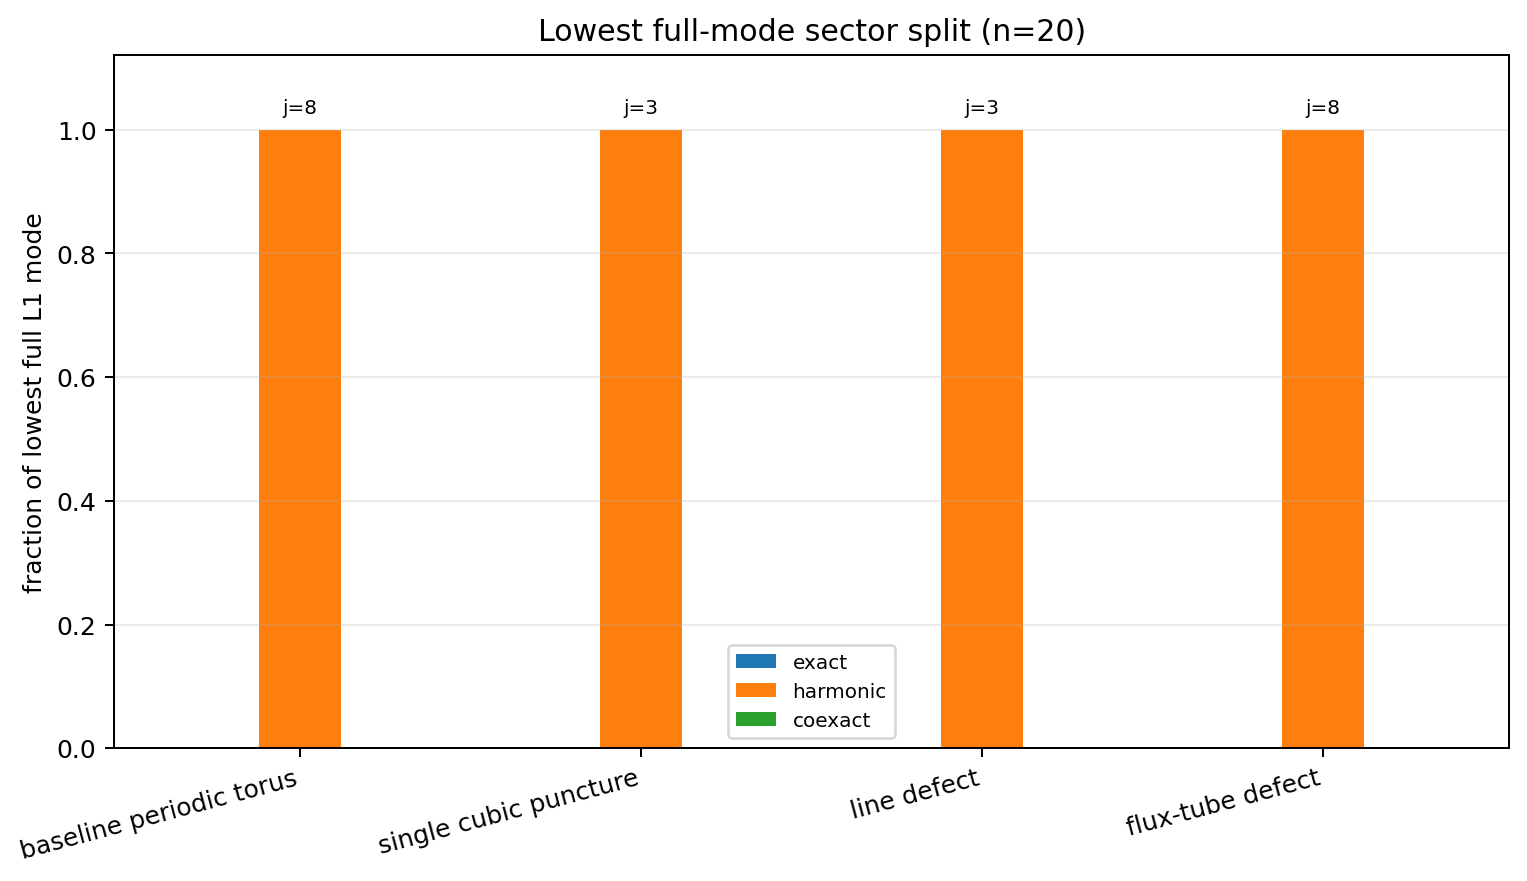
\includegraphics[width=0.48\linewidth]{../plots/20260412_141530_transverse_sector_split.png}
\caption{CP2 vector diagnostics. Left: restricted low transverse spectrum compared with the continuum ordering. Right: explicit harmonic/coexact split showing that the true low full-spectrum floor remains harmonic while the projected transverse branch lives above it.}
\label{fig:cp2}
\end{figure}

\section{CP2b and CP2c: Deeper Window Scans and Gap Scaling}

\subsection{Defect-assisted isolation}

The next step was to deepen the full-spectrum scan window and test whether defects pull a genuinely coexact branch earlier into the low spectrum. The $n=20$ CP2b scan showed:
\begin{itemize}
\item baseline first strong coexact candidate at $j=11$ with coexact fraction $0.849$;
\item puncture first strong coexact candidate at $j=3$ with coexact fraction $1.000$;
\item line defect first strong coexact candidate at $j=3$ with coexact fraction $1.000$;
\item flux tube first strong coexact candidate at $j=11$ with coexact fraction essentially $1.000$ and the strongest defect localization in that scan, near-defect fraction $0.021$.
\end{itemize}

That is a meaningful improvement in sector isolation. Defects do help separate the coexact branch from the harmonic floor. But even at this stage the floor itself remained harmonic.

\subsection{Direct harmonic-to-coexact gap scaling}

CP2c made the diagnostic more direct by measuring the gap between the true full-spectrum floor and the first strong coexact candidate across $n=12,16,20,24,28$. Table~\ref{tab:cp2c-n28} records the largest-size result.

\begin{table}[t]
\centering
\small
\begin{tabular}{lccccc}
\toprule
Branch & candidate $j$ & coexact frac & scaled gap & near-defect frac & restricted/candidate \\
\midrule
baseline & 19 & 0.806 & 78.376 & 0.002 & 0.500 \\
puncture & 3 & 1.000 & 38.870 & 0.001 & 1.000 \\
line defect & 3 & 1.000 & 38.871 & 0.000 & 1.000 \\
flux tube & 11 & 1.000 & 39.192 & 0.011 & 0.965 \\
\bottomrule
\end{tabular}
\caption{Largest-size CP2c gap-scaling result at $n=28$. Defects compress the harmonic-to-coexact separation and improve localization, but the gap does not collapse to zero.}
\label{tab:cp2c-n28}
\end{table}

The clean baseline is especially informative. For $n=16,20,24$ its scaled gap stays near $38.6$--$39.1$, and at $n=28$ the first threshold-passing coexact candidate moves deeper to $j=19$, producing a larger scaled gap of $78.376$ with projected-to-candidate ratio $0.500$. Whatever the detailed family interpretation of that deeper transition, it is not evidence that the harmonic floor is collapsing into a clean low coexact continuum band. It is evidence of continued separation.

The defected branches remain more favorable:
\begin{itemize}
\item puncture and line defect keep the first strong coexact candidate at $j=3$ through the tested larger sizes;
\item puncture gives the smallest $n=28$ scaled gap, $38.870$;
\item flux tube gives the strongest $n=28$ localization signal, near-defect fraction $0.011$.
\end{itemize}

This is enough to support a bounded CP2c statement:
\begin{quote}
defects compress the harmonic-to-coexact separation and can isolate the coexact branch much earlier in the low window, but they do not yet turn that coexact branch into the actual low propagating floor of the full $L_1$ spectrum.
\end{quote}

\begin{figure}[t]
\centering
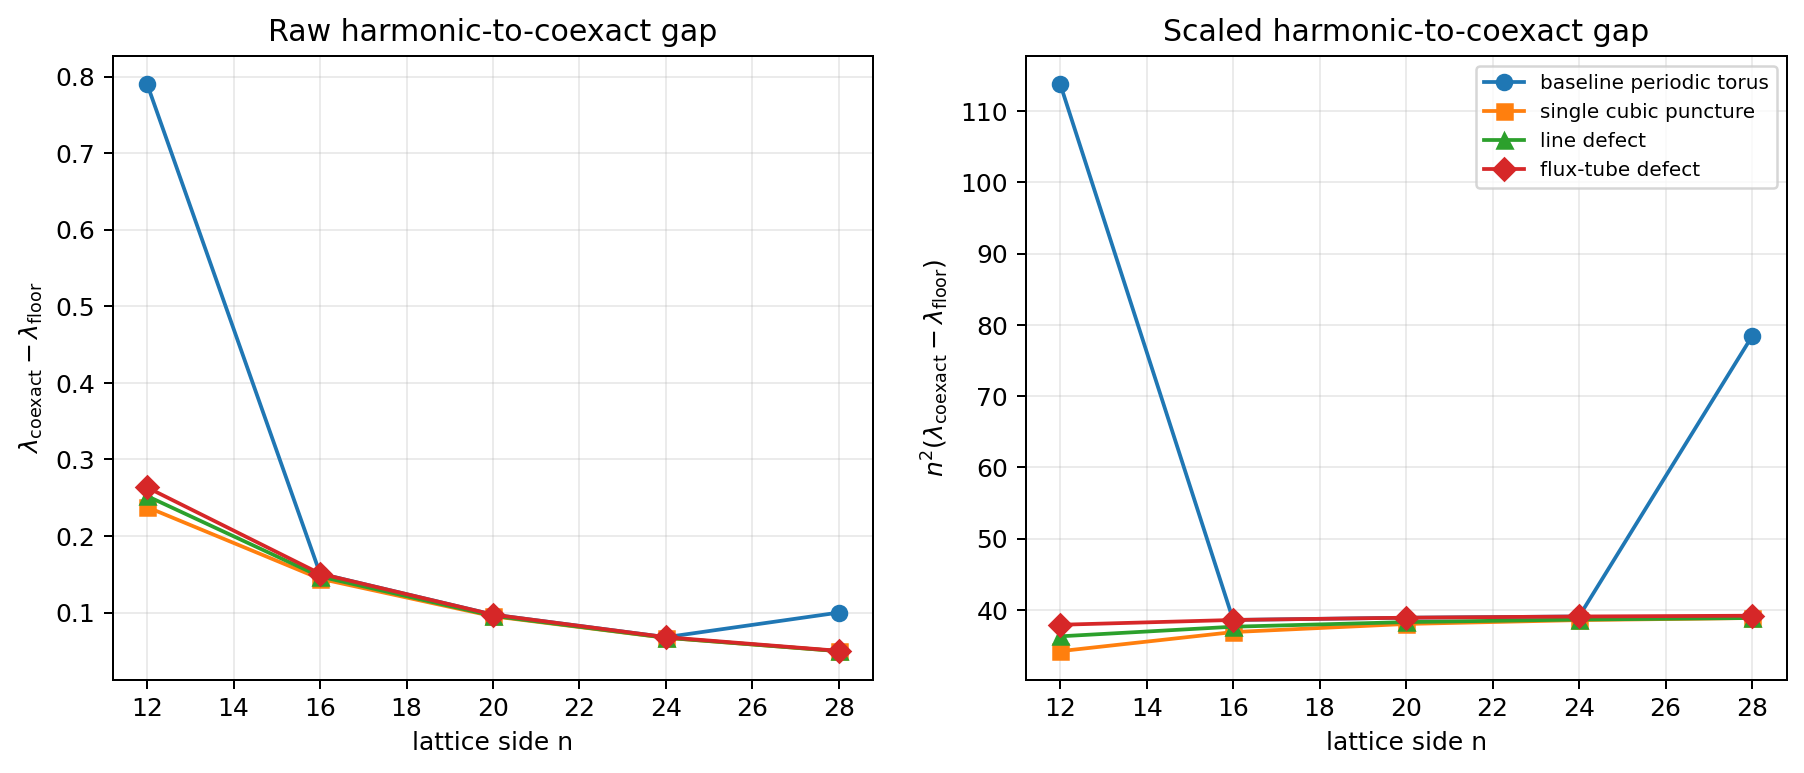
\includegraphics[width=0.48\linewidth]{../plots/20260412_144123_transverse_sector_gap.png}
\hfill
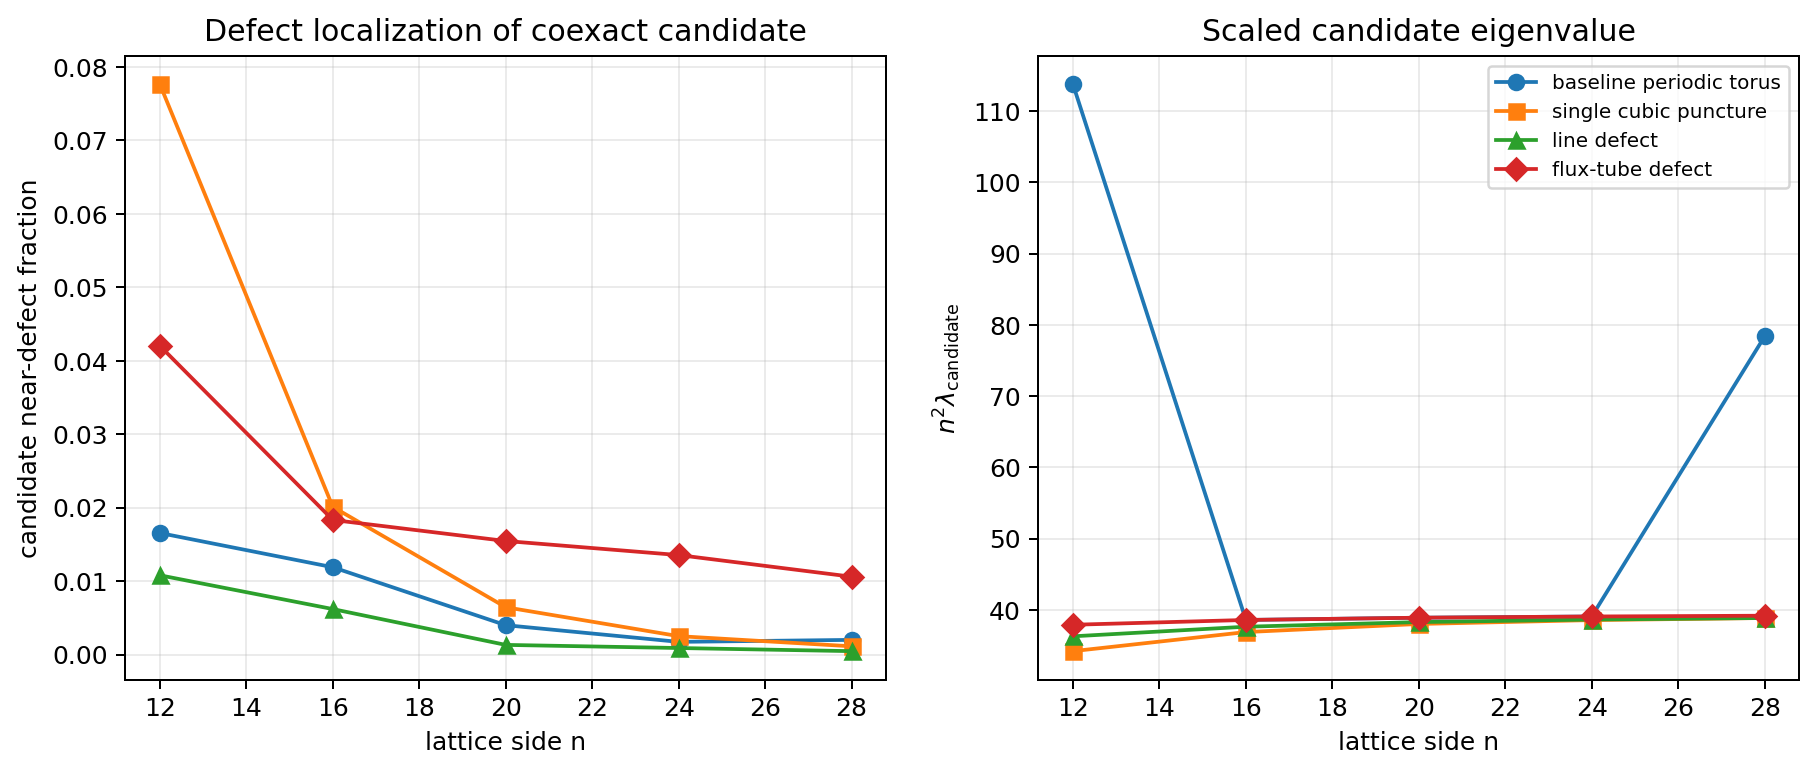
\includegraphics[width=0.48\linewidth]{../plots/20260412_144123_transverse_sector_localization.png}
\caption{CP2c diagnostics. Left: direct harmonic-to-coexact gap across refinement and defect backgrounds. Right: localization of the selected coexact candidate near the defect support.}
\label{fig:cp2c}
\end{figure}

\section{Current Authority Boundary}

After CP1 through CP2c, the repository now supports the following bounded statements.

\subsection{Established}

\begin{enumerate}
\item The scalar node operator has a real continuum-control contract in the tested local-kernel regime. It survives the cubic interior scan, weakly perturbed point sets, and reflected Dirichlet and Neumann boundary controls.
\item The restricted transverse branch remains a meaningful coexact sector. After projection, its low spectrum still follows continuum ordering and scale patterns in the tested periodic and defected backgrounds.
\item The full-spectrum vector question is now better diagnosed than before. The actual low $L_1$ floor remains harmonic, and the harmonic-to-coexact gap stays finite in the tested window.
\item Defects are not irrelevant perturbations. They can pull the coexact branch deeper into the low spectrum and increase localization in a controlled way.
\end{enumerate}

\subsection{Not established}

\begin{enumerate}
\item A true low continuum vector floor on the full $L_1$ spectrum.
\item Maxwell dynamics, gauge theory, photon interpretation, or quantum-field interpretation.
\item Universality across broad kernel families, substrate families, or defect families.
\item Metric closure, curvature extraction, or a closed geometric field picture from the same continuum operator family.
\end{enumerate}

The interpretation boundary is therefore sharp. HAOS-IIP now has a stronger scalar continuum foothold and a clearer vector obstruction. It does not yet have a closed continuum-physics theory.

\section{Detailed Future Plans}

The next program should shrink to the unresolved structure rather than expand the claim language. A disciplined sequence is:

\begin{enumerate}
\item \textbf{CP2d: harmonic-floor resolution.} The immediate task is to determine what the harmonic low floor actually is on the tested backgrounds. That means explicit quotienting or classification of the harmonic/topological sector, careful tracking of torus-cycle content under defects, and a test of whether one can define a stable coexact propagating window \emph{after} that floor is removed rather than merely above it. Success would be a refinement-stable coexact branch whose low edge is no longer contaminated by unresolved harmonic structure.

\item \textbf{CP3: effective-law closure.} The late frozen phases already provide propagation, ordering, causal-closure, and distance-surrogate observables. The next contract is to fit those observables to a compact family of continuum closures such as diffusion-like, wave-like, or advection-diffusion forms and to require coefficient stability under refinement and branch/control comparison. Success would mean one small law family organizing the late-phase data without repeated retuning.

\item \textbf{CP4: geometry closure.} The scalar continuum foothold and the late distance-surrogate diagnostics need to be tested against one common effective geometry reconstruction. This should proceed through Green-response, heat behavior, shell-arrival slopes, and low-mode organization under the same metric-like coarse reconstruction. Success would mean one effective geometry organizing both the scalar operator and the late-phase surrogate diagnostics.

\item \textbf{CP5: universality contract.} None of the present results should be promoted to ``continuum physics'' unless the same low-energy statement survives controlled changes of kernel width, substrate family, defect family, and coarse-grain map. This stage should explicitly compare local-kernel stability against modest kernel variations and alternate substrate families rather than relying on one tuned branch.

\item \textbf{CP6: first-order and integrated sector synthesis.} Only after CP2d through CP5 should the first-order or Dirac-like sector be reintroduced into a continuum-scaling story. The target is not particle language. The target is a coherent operator family in which scalar, coexact vector, and first-order sectors can be described on one compatible continuum side without importing ontology from outside the measured hierarchy.
\end{enumerate}

These steps also define the failure boundary. If CP2d fails, the vector claim must shrink back to ``projected coexact branch above a harmonic floor.'' If CP3 fails, the late phases remain kinematic rather than equation-bearing. If CP4 fails, geometry stays surrogate-level. If CP5 fails, the whole continuum picture remains branch-specific. Those are acceptable outcomes; they are exactly what the program is meant to test.

\section{Conclusion}

The repository is farther along than the older startup notes suggested, but the present answer is still bounded. CP1 now passes as a genuine scalar continuum-control result in the local-kernel regime. CP2 through CP2c then sharpen the vector picture: the projected transverse branch remains continuum-like after projection, yet the true low full-spectrum $L_1$ floor is still harmonic, and the direct harmonic-to-coexact gap does not collapse in the tested window. Defects help isolate the coexact sector, but they do not yet convert it into the actual low propagating floor.

The honest synthesis is therefore simple. HAOS-IIP now has:
\begin{enumerate}
\item a stronger scalar continuum contract;
\item a real but still obstructed coexact vector branch;
\item a disciplined future program for deciding whether those ingredients can be closed into a broader continuum-physics statement.
\end{enumerate}

That is enough for a numbered synthesis release. It is not yet enough for continuum ontology.

\section*{Project Resources}
Project website: \url{https://tomislav-rupic.com/}

Code repository: \url{https://github.com/tomislavrupic}

Archived release (Zenodo DOI): \url{https://doi.org/10.5281/zenodo.18938323}

\end{document}
